\chapter{Synchronization}
\section{Semaphores}

Proposed by Dijkstra, Semaphores are special counters on which 2 operations are defined :
\begin{itemize}
  \item P or wait on a semaphore s :
    \begin{verbatim}
      if (s.counter == 0)
        wait
        s.counter--
    \end{verbatim}
  \item V or post on a semaphore s :
  \begin{verbatim}
      s.counter++
  \end{verbatim}
\end{itemize}

\subsection{Typical use :} 

\begin{itemize}
  
\item restrict the access to a region to a fixed number of threads.
Example :

\begin{verbatim}
    s = semaphore initialized to N
    threads execute :
        wait(s);
            restricted section;
        post(s);
\end{verbatim}

\item as a lock (binary semaphore).
Example :
\begin{verbatim}
  s = semaphore initialized to 1
  Some code as above for threads.
\end{verbatim}
\end{itemize}

\subsection{Example: Procuder/Consumer}

\begin{figure}
  \begin{center}
    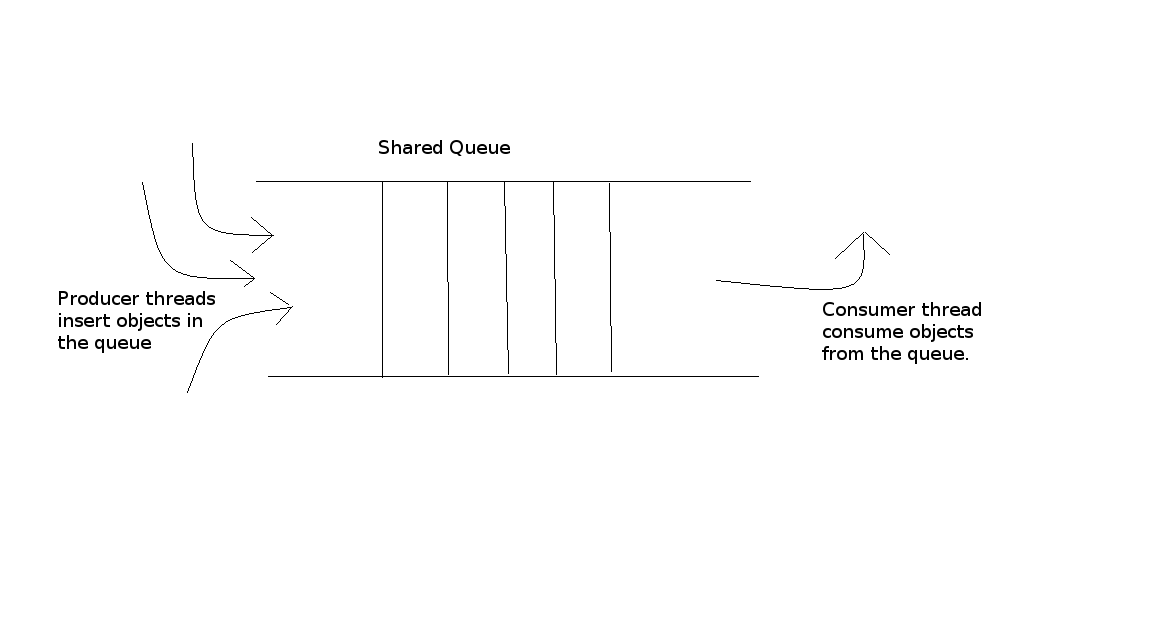
\includegraphics[scale=0.5]{shared_queue.png}
    \caption{Situation of the producer/consumer example}
    \label{}
  \end{center}
\end{figure}

In this example, we will use a circular buffer of size N as our queue.
If an operation is not possible, threads wait until the operation is possible.
\begin{verbatim}
semaphore s = 1, available = N, occupied = 0;

produce(int object) {

     //possibility to wait
     wait(available);
     // at most N producers
     wait(s);
     queue.buffer[(queue.head + queue.size) % N ] = object;
     queue.size++;
     post(s);
     post(occupied);
}

int consume() {
     int result;
     wait(occupied);
     // number of consumers waiting bounded...
     wait(s);
     result = queue.buffer[queue.head];
     queue.head = (queue.head +1) % N;
     queue.size--;
     post(available);
     post(s);
}
//Idea : use semaphores to count :
// the number of available slots (semaphore initialized to N)
// the number of occupied slots (semaphore initialized to 0)

Comment on the code: complicated because the order of wait operation matters.
\end{verbatim}



\subsection{Implementation of Semaphores :}

A semaphore is :
\begin{itemize}
  \item an integer value : counter
  \item a list of blocked processes : l
  \item a boolean variable : lock
\end{itemize}
\begin{verbatim}
  typedef struct{
  int lock;
  list l;
  int counter;
  } semaphore_t;
  
  // initially, lock=0, l is empty, counter is defined at semaphore creation
  
  void wait(semaphore_t s){
       while(test_and_set(&s.lock,1) {}
       if (s.counter>0){
            s.counter--;
            s.lock =0;
       }
       else{
            tid = get_current_thread_id();
            unschedule(tid);
            mark_as_blocked(tid);
            insert(s.l,tid);
            s.lock = 0;
            schedule();
       }
  }
  
  void post(semaphore_t s) {
       while(test_and_set(&s.lock,1) {}
       if (is_empty(s.l)){
            s.counter++;
            s.lock =0;   
       }
       else {
            tid = remove(s.l);
            mark_as_unblocked(tid);
            s.lock = 0;
       }
  }
  
  Comment : the wait operation takes advantage of the scheduler to perform its task.
\end{verbatim}

\section{Monitors}

Introduced by Haare, monitors are objects in which methods are executed in mutual exclusion.

\begin{tabular}{cccc}
  threads & \vdots & \vdots & \vdots
\end{tabular}
|
| 
\textgreater
\begin{tabular}{|c|}
 attributes \\
 : \\
 : \\
 : \\
\end{tabular}

Only one thread at a time can execute something inside the monitor .

This model makes things simpler because it is not necessary to manage locks anymore.

\subsection{Example: Producer/Consumer}

The queue will be implemented as a monitor, with buffer, size, head as attributes and two methods :

Thr monitors support two operations :
\begin{itemize}
  \item wait(condition C) : releases the access to the monitor then waits until some signal is sent on C, then compete for the lock to retrieve access to the monitor.
  \item signal(condition C) : sends a signal on C. The signal is lost if no thread waits on C.
\end{itemize}
 
 
 \begin{verbatim}
 
  condition not_full , not_empty;
  
   produce(int object){
        while(size==N)
        wait(not_full);
        buffer[(head+size)%N] =object;
        size++;
        signal(not_empty);
   }
   
   int consume(){
        int result;
        while(size==0)
        wait(not_empty);
        result = buffer[head];
        head =(head+1)%N;
        size--;
        signal(not_full);
   }
 \end{verbatim}


\subsection{Implementation}

Similar to semaphores. Notice that both models are equivalent. It is possible to implement one of them using the other.
